\section{Theory}
%\subsection{Basic theory of grating spectrometer}




%\subsection{Optical Fiber / brewster angle}

\subsection{Light emission and absorbtion}

The electron of an specific atom has a discrete spectrum of energy-levels determined by the potential of the nucleus and the other electrons. When light interacts with an atom, we are essentially adding energy to the atom, due to the energy associated with light of a certain frequency $f$ $E=hf$. Due to the quantum nature of light and electrons, only light of a frequency corresponding to the difference in energy between to of the discrete energy levels of the atom can move the from the lower energy level to the upper. This process is called absorbtion, and if we send light at an material, the material will absorb light of the wavelengths corresponding to energy transitions of the chemical element composure of the material. Likewise, when the electron transitions back to a lower energy state, the atom will emit a photon with a frequency corresponding to the transition energy, which is called emission. Like with absorbtion, each material will emit light at frequencies corresponding to it's chemical element composition. On can measure the spectrum of an material either absorbing or emitting light, and determine the energy transistions by looking at the spectral lines of the spectrum. For the absorbtion spectrum this will be minima on a wavelength vs. intensity graph. \\

The lines that exist due to the differences in the allowed quantum states will have a even finer splitting due to fine and hyperfine structure, which arises due to the dipole moment of the electron and the nucleus respectively. 


\subsubsection{Blackbody radiation}
All matter emits electromagnetic radiation, when it has a temperature above absolute zero. This radiative distribution of entropy is called thermal radiation and is a spontaneous process.

Similarly, all matter absorbs electromagnetic radiation to some degree. In addition, a blackbody is an object that absorbs all radiation of all wavelengths that falls upon it. Furthermore, at thermal equillibrium a blackbody emits a characteristic frequency distribution, which is temperature depended. The relationship between the spectral radiance density $B_f$ for a certain frequency $f$ and the temperature of a black body is given by plancks law:

\begin{align}
B_{f}(T)= \frac{2hf^3}{c^2}\frac{1}{\exp(\frac{hf}{kT})-1}
\label{planck}
\end{align}

Where $c$ is the speed of light, $h$ is Planck's constant, $k$ is Boltzmann's constant and $T$ is the temperature. For each frequency or wavelength $\lambda$ (related by $\lambda f = c$), there is a certain temperature where the spectral radiance density will reach its maxima or wise versa, eg. for each temperature there is a characteristic wavelength were the spectral radiance density has a maxima. The relationship between this temperature and wavelength is inversely proportional, and is given by Wien's displacement law:

\begin{align}
\lambda_{max}T=b
\label{wien}
\end{align}

Where $b$ is Wien's displacement constant, which has a value of $\SI{2.897 e-3}{\kelvin \meter}$. 


\subsection{Light bulbs and the solar spectrum}



\begin{figure}[h!]
    \centering
    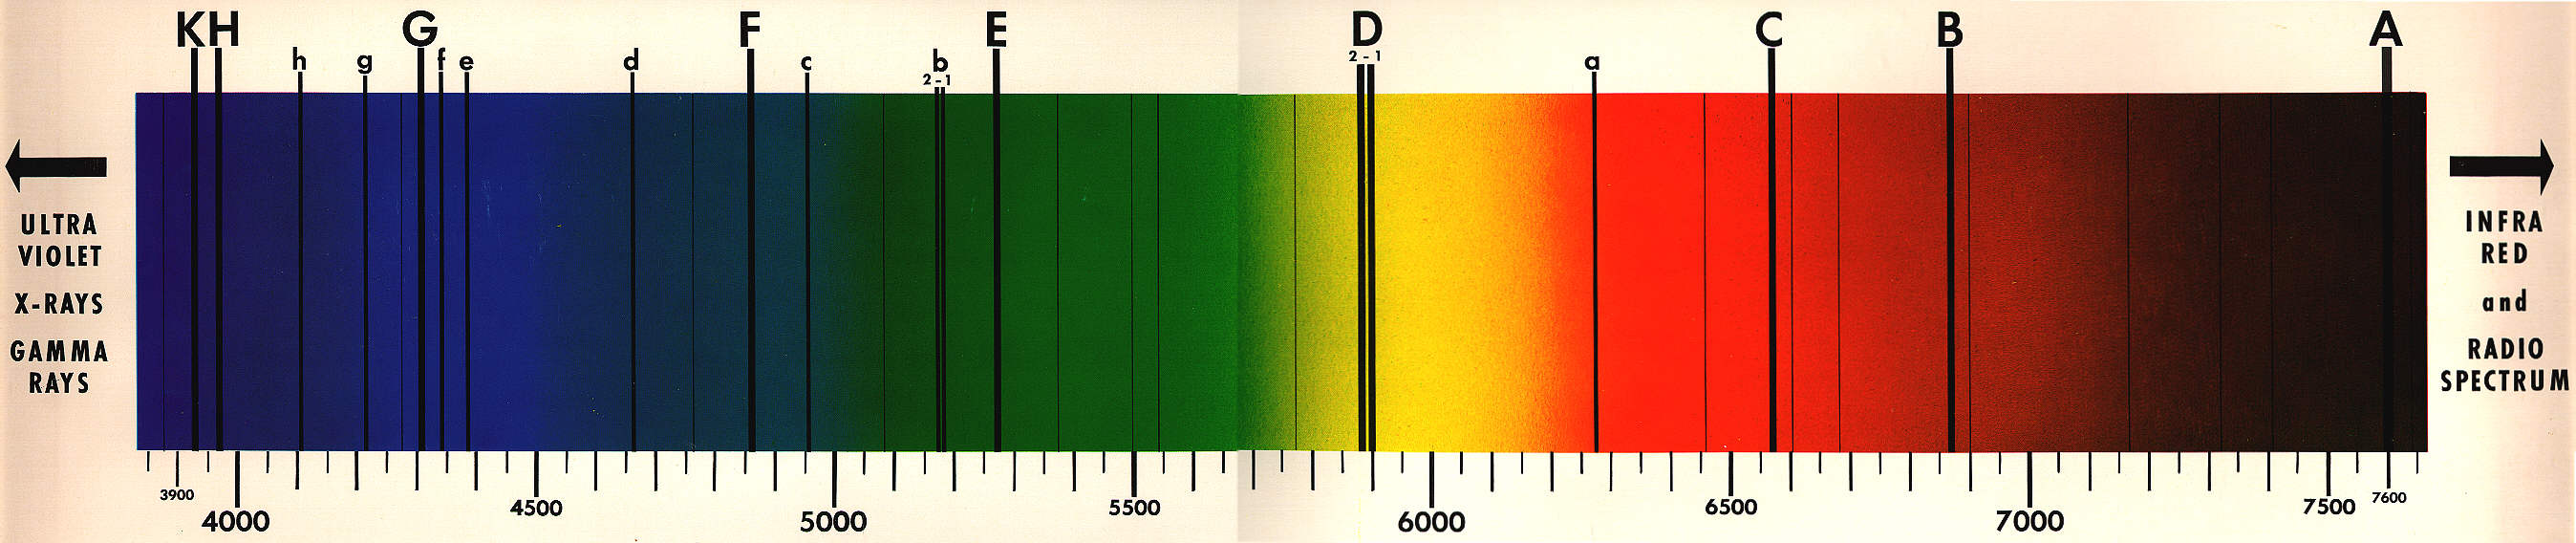
\includegraphics[width=0.5\textwidth]{solarspectrum}
    \caption{The solar spectrum}
    \label{fig:solarspectrum}
\end{figure}

Wiens displacement law

\begin{equation}
    \lambda_{\text{peak}}T = \SI{2.898e-3}{\meter\kelvin} \label{eq:wien}
\end{equation}

\begin{table}
	\begin{tabular}[h]{ccc}
		\toprule
		\multicolumn{3}{c}{title}\\
		\midrule
		Obs. Wavelength & Lower level & Upper level  \\
		\multirow{2}{*}{462} & 12  & 6 \\
		 & 8 & 9 \\
		\bottomrule
	\end{tabular}
\end{table}
